% !TeX document-id = {a24bb292-b05f-4465-9a19-f6adbf8b8362}
%% A simple template for a term report using the Hagenberg setup
%% based on the standard LaTeX 'report' class
%%% äöüÄÖÜß  <-- no German umlauts here? Use an UTF-8 compatible editor!

%%% Magic comments for setting the correct parameters in compatible IDEs
% !TeX encoding = utf8
% !TeX program = pdflatex 
% !TeX spellcheck = en_US
% !BIB program = biber

\RequirePackage[utf8]{inputenc} % Remove when using lualatex or xelatex!
\RequirePackage{hgbpdfa}        % Creates a PDF/A-2b compliant document

\documentclass[english,notitlepage,smartquotes]{hgbreport}
% Valid options in [..]: 
%    Main language: 'german' (default), 'english'
%    Turn on smart quote handling: 'smartquotes'
%    APA bibliography style: 'apa'
%    Do not create a separate title page: 'notitlepage'
%%%-----------------------------------------------------------------------------

\graphicspath{{images/}}  % Location of images and graphics
\bibliography{references} % Biblatex bibliography file (references.bib)

%%%-----------------------------------------------------------------------------
\begin{document}
%%%-----------------------------------------------------------------------------

\author{Tobias Kothbauer, Veronika Leitner}                    % Your name
\title{Guide Guru - Interactive Travel Guide Project Report}	                 % or "Project Report"
\date{\today}

%%%-----------------------------------------------------------------------------
\maketitle
%%%-----------------------------------------------------------------------------

\begin{abstract}\noindent
In the dynamic landscape of modern travel, Guide Guru emerges as a individual solution, poised to redefine the way users embark on their adventures. Rooted in the fusion of cutting-edge technology and user-centric design philosophy, this project endeavors to craft a travel guide application that avoids limitations of traditional planning methods. 

\bigskip
\noindent At its core, Guide Guru is driven by the vision of empowering travelers with a personalized experience, one that seamlessly aligns with their interests, preferences and hobbies. Leveraging the capabilities of advanced large language models, the application will function as an intuitive digital companion, which adapts to the desires of each user. By fostering a tight relationship between technology and user input, Guide Guru endeavors to simplify the travel planning process, offering a platform where every journey is curated to reflect the personality of the individual. 

\bigskip
\noindent
\end{abstract}

%%%-----------------------------------------------------------------------------
\tableofcontents
%%%-----------------------------------------------------------------------------

%%%-----------------------------------------------------------------------------
\chapter{Aims and Context}
%%%-----------------------------------------------------------------------------

The core objective of this project is to develop an intuitive and adaptable travel guide application that seamlessly integrates user input with language processing capabilities. Through the implementation of user surveys, Guide Guru should gather and evaluate individual interests, ensuring that every travel recommendation is finely tuned to match the user's specific desires and hobbies.

The envisioned application gives users a tool with a simple interface, allowing them to effortlessly select destinations and specify personal interests, thereby generating travel guides curated to their liking.

Moreover, Guide Guru will offer the practical functionality of exporting personalized guides in PDF format, enabling users to conveniently access their curated recommendations on various devices and platforms.

Upon completion, Guide Guru targets delivering a travel companion, that eases the planning process and allows a high levels of customization and efficiency. By placing the user at the center of the experience, Guide Guru aims to enhance the quality of travel adventures, empowering individuals to craft marvelous journeys that align, with their interests and preferences.

In order to accurately reflect user preferences in Guide Guru, a questionnaire was created. Thirty-three participants provided insights into their travel habits, hobbies, interests, and their perspectives on the ideal format for a travel guide. This data has allowed us to customize Guide Guru to cater to a diverse audience, requiring minimal user input while still meeting their needs effectively.

%%%-----------------------------------------------------------------------------
\chapter{Project Details}
%%%-----------------------------------------------------------------------------
%Describe important project steps, \eg, the rationale of the chosen architecture
%or technology stack, design decisions, algorithms used, interesting challenges
%faced on the way, lessons learned \etc
Throughout our project, we meticulously navigated various crucial steps to guarantee the success and deliver high-quality results for our Guide Guru. From designing comprehensive surveys to selecting optimal technology stacks, our journey was marked by strategic decisions aimed at creating a personalized and effective travel guide experience.

\section{Questionaire}

Initially, we developed a questionnaire based on our understanding of the essential information required to create a straightforward yet impactful prototype with highly personalized outcomes.

This survey encompassed inquiries into user preferences, evaluations of the relevance of various travel aspects, and free text questions to glean insights into relevant hobbies and desired content for the travel guide.

Key findings from the survey revealed that the majority of participants preferred selecting their destination rather than receiving recommendations. Primary considerations for their travels included the type of travel (\eg, relaxation vacation), the overall environment (\eg, beach or city), and the preferred season for travel. Discovering new hobbies ranked as the least important aspect. All participants expressed a preference for receiving the travel guide in PDF format, with a strong emphasis on the importance of suitable images. Additionally, 85\% favored selecting their hobbies from a predefined list, with sports and art \& culture emerging as the most frequently mentioned categories. Regarding desired information in the travel guide, participants highlighted sights and hidden gems, culinary recommendations, entertainment options, cultural insights, and information on country-specific risks and hazards.

\section{Technology Stack}
Simultaneously, we conducted research on potential technology stacks. Two components were predetermined: utilizing React\footnote{https://react.dev} for frontend development to enhance our web development skills with this technology, and selecting ChatGPT from OpenAI\footnote{https://openai.com} as our preferred large language model (LLM), thus our supervisor thankfully could provide us with an API key for this model.

Following several iterations, we opted to employ Python\footnote{https://www.python.org} for backend development after discovering its well-documented approach to integrating a LLM into a web application. As well Flask\footnote{https://flask.palletsprojects.com/en/3.0.x/}, a micro web framework, was chosen to handle requests and CORS policies.

Given the importance of images as indicated by survey participants, and considering the multitude of cities and places of interest generated by user input, we needed a means to access online data for countless locations. To achieve this, we utilized a combination of the Google Places API\footnote{https://developers.google.com/maps/documentation/places/web-service/overview?hl=de} and Google Photos API\footnote{https://developers.google.com/photos?hl=de} to download and display images from user recommendations, providing users with a simple yet effective insight into selected destinations.

To validate user input for potential travel destinations, we integrated the geonames API\footnote{https://www.geonames.org}, which is user-curated and lists millions of places, allowing filtering for highly populated areas. This API facilitated the inclusion of destinations with populations exceeding 1000, ensuring a diverse range of travel destinations could be used to generate the guide.

\section{Prototype Design}

\begin{figure}
	\centering
	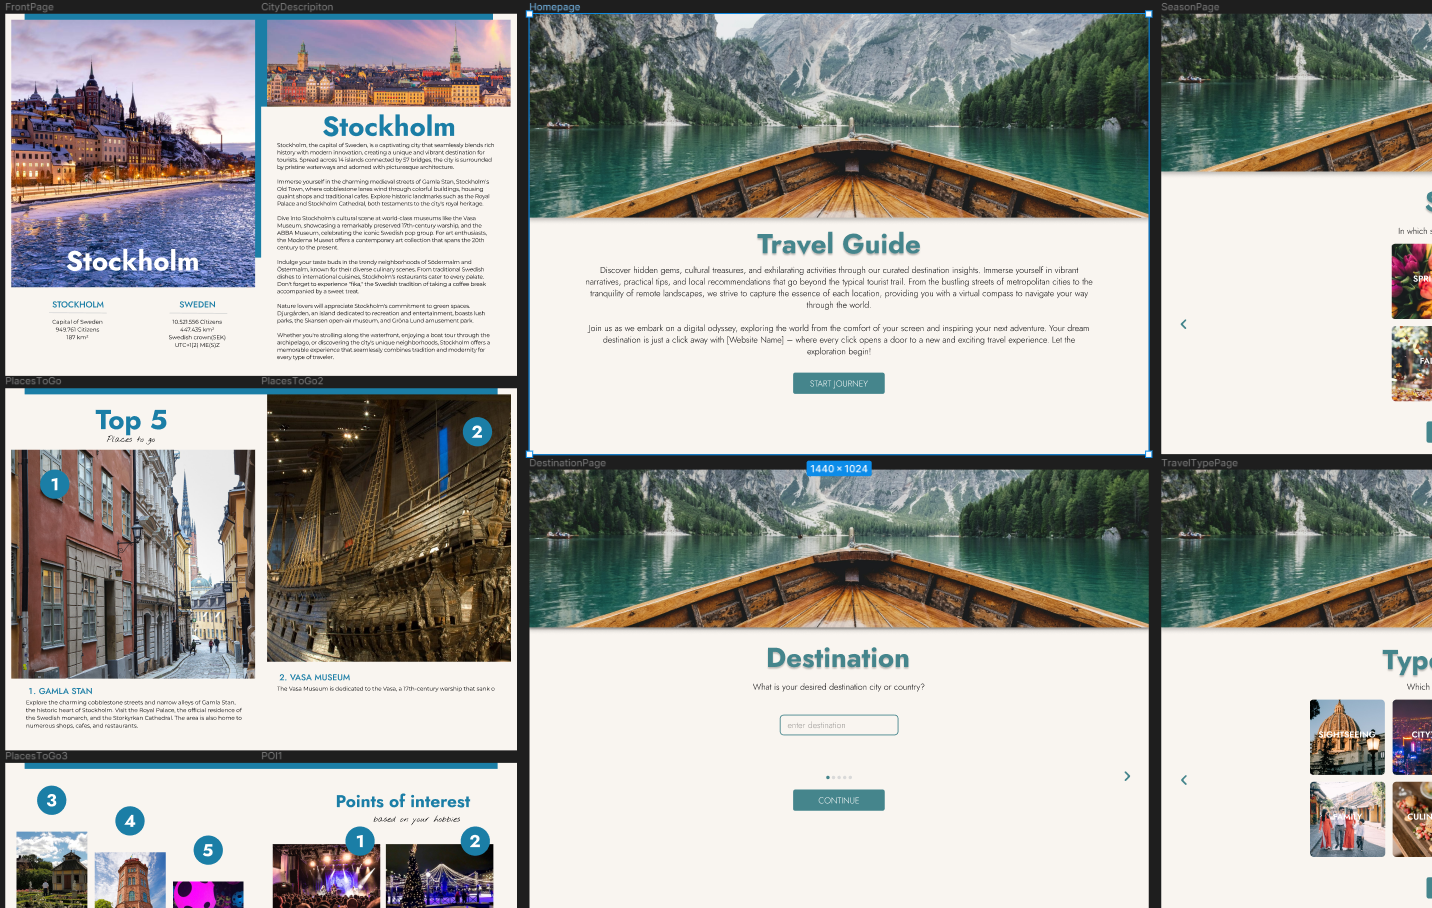
\includegraphics[width=1\textwidth]{Mockup_Example.png}
	\caption{Mockup of Applicaton and Guide}
	\label{fig1}
\end{figure}

Equipped with insights gleaned from our survey, we embarked on the development of an initial mockup for Guide Guru. Leveraging Figma\footnote{https://www.figma.com/de}, a collaborative design tool, we crafted a clickable prototype encompassing the entire user journey and a blueprint for our PDF guide. This mockup (see figure  \ref{fig1}) enabled us to pinpoint necessary input parameters, map out pages, identify reusable components, and discover the inherent structure of our web application in a fast and efficient manner.


\section{Implementation First Prototype}
 

\section{User Testing}


\section{Final Prototype}

\section{Challenges}


\section{Lessions Learned}



%%%-----------------------------------------------------------------------------
\chapter{System Documentation}
%%%-----------------------------------------------------------------------------

%Give a well-structured description of the architecture and the technical design
%of your implementation with sufficient granularity to enable an external person
%to continue working on the project.

\section{Backend}

\subsection{Large Language Model Integration}

\subsection{Integration of Google APIs}

\subsection{Geonames API for Destinations}

\section{Frontend}

\subsection{Pages}

\subsection{Components}

\subsection{React PDF}

%%%-----------------------------------------------------------------------------
\chapter{Summary}
%%%-----------------------------------------------------------------------------

Give a concise (and honest) summary of what has been accomplished and what not. 
Point out issues that may warrant further investigation.

%%%-----------------------------------------------------------------------------
\appendix                                                   % Switch to appendix
%%%-----------------------------------------------------------------------------

%%%-----------------------------------------------------------------------------
\chapter{Supplementary Materials}
%%%-----------------------------------------------------------------------------

The appendix is a good place to attach a user guide, screenshots, installation
instructions, etc. Add a separate chapter for each major item.

%%%-----------------------------------------------------------------------------
\MakeBibliography[nosplit]
%%%-----------------------------------------------------------------------------

%%%-----------------------------------------------------------------------------
\end{document}
%%%-----------------------------------------------------------------------------
